\chapter{Background and Related Works}
\label{ch:background}
This chapter introduces the basic concepts and relevant techniques involved in this project, including stock market, stock market data, time-series analysis, machine learning, data clustering, representation learning, nerual networks. In addition, representative works that are related to this project are reviewed.

\section{Stock Market and Stock Market Data}
A stock is a term used to describes the partial ownership certificates of any company, while a share represents the stock certificate of a particular company. Given the two terms, a stock market can be regarded as a place for the transfer, trading and circulation of issued shares. Because it is based on the issuance market, stock market is also called the secondary market. A stock exchange is a subset of a stock market, but they are usually used interchangeably. New York Stock Exchange (NYSE), Nasdaq, and the Chicago Board Options Exchange (CBOE) are three most well-known stock exchanges in the stock market of the U.S. For companies, stock markets are the main place to raise necessary capital from investors. For investors, they can get returns from their shares. \\
\\Every action in stock markets can be treated as stock market data, but in reality, merely the prices and trades information of shares are recorded. Those information are often studied by investors, traders and researchers for making better decision. Investors and traders make use of the data to decide the shares buying and selling, they try to predict the future movement of the prices to avoid risks and make more profit. Researchers use those data to make assumptions and test their hypothesis.\\
\\In the past, stock data were collected and recorded by financial data vendors. After information technological revolution, those data are manipulated and stored automatically by computers. Through the Internet, basic information such as the open price, closing price, exchange code are public accessible. Figure~\ref{fig:yahoo1} shows an sample of stock market data from Internet.\\
\begin{figure}[!htbp]
    \centering
    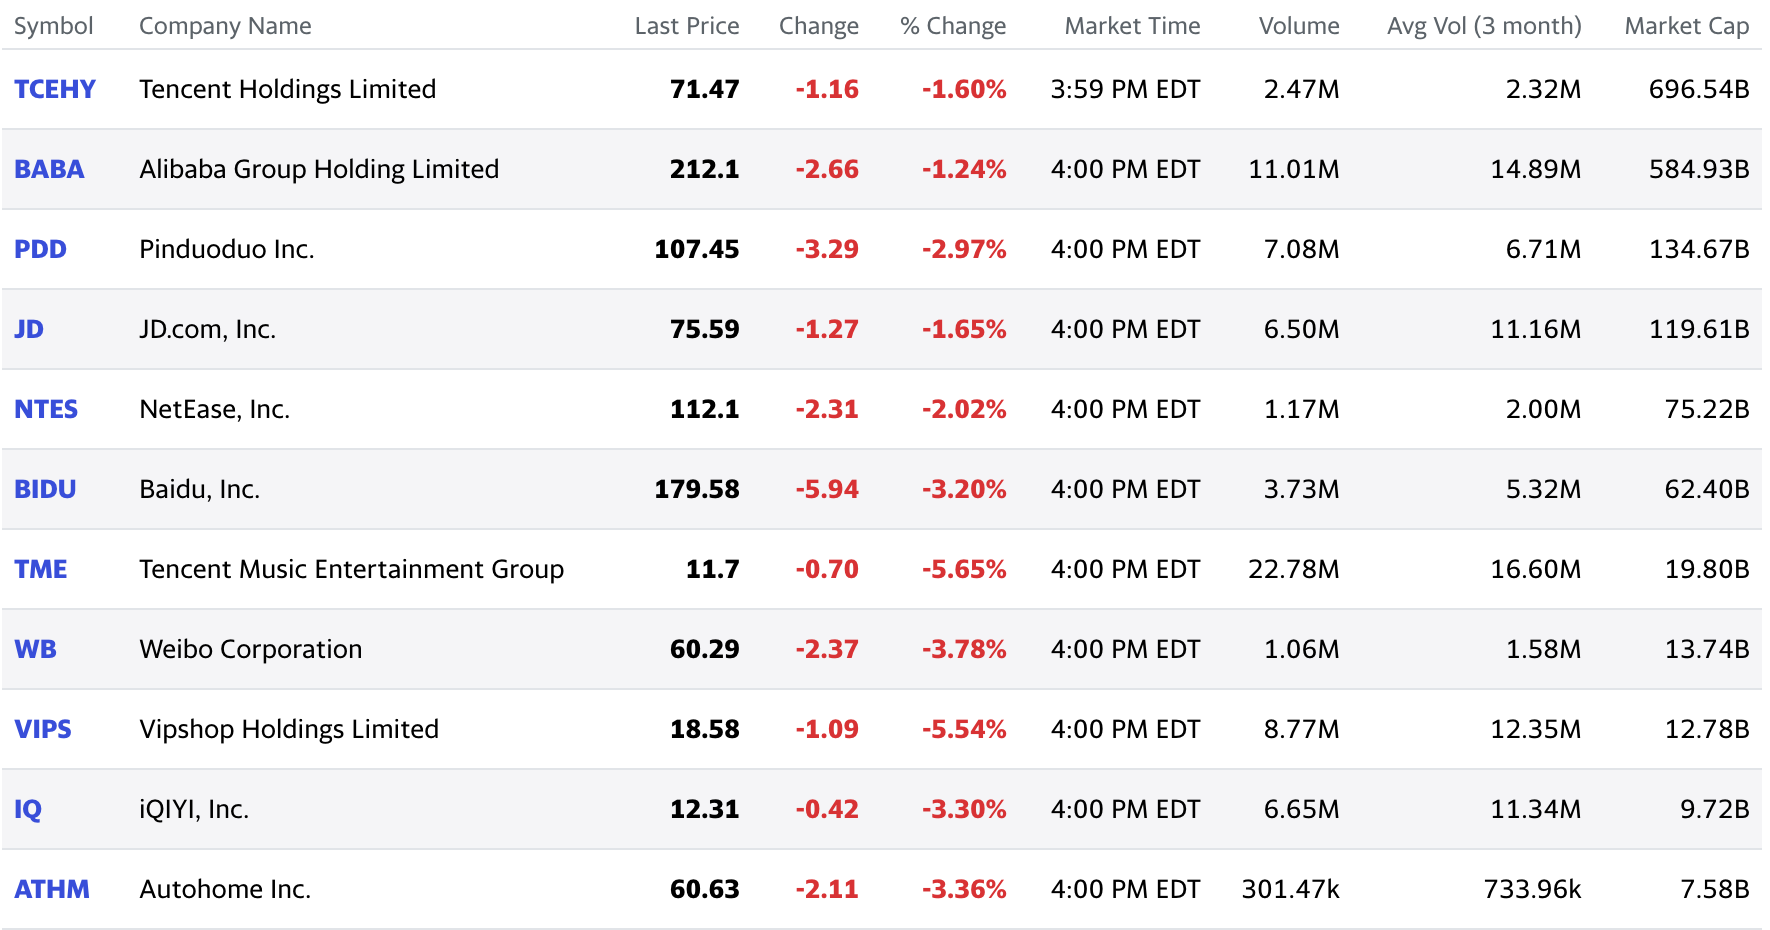
\includegraphics[width=0.8\columnwidth]{yahoo.png}
    \caption{Sample of stock market data from \href{https://finance.yahoo.com/}{Yahoo}}
    \label{fig:yahoo1}
\end{figure}
\\Stock market data can be stored and transfered with various data model, in reality, they are mostly in the form of time-series data, meaning that there is always a time axis with it. This project mainly studies on the price sequences of stocks and therefore can be categorized into time-series analysis taks.

\section{Time-Series Analysis for Stock Market Data}
\subsection{Time-series data}
According to \cite{davis2014introduction}, time-series data are a collection of observations extracted repetitively at continuous specific time points. Given a small sampling interval, the dimension of time-series data could be extremely large. In addition, in time-series data, each data point is numerical. These two facts show the basic properties of time-series data: numerical, continues and high-dimensional. Apart from stock market data, there are numerous data are in the form of time sequence, such as the voice data and video data.\\
\\Generally, analysis of time-series data can be used in following four applications: (1) sequence data compression; (2) influential factor revelation; (3) pattern identification; (4) sequence prediction. Sequence data compression aims to find a way to compress data while preserve the most information, it can benefit the data storage. Influential factor revelation aims to find the for sequence change, it can be used in abnormality discovery. Pattern identification aims to extracting common phenomena existing in different sequences, it can be used in sequence comparison. Sequence prediction aims to predict the future trend of sequences based on the historical data, it can be used in decision making. Apart from those applications, researchers can seek help from time-series analysis to explain finacial phenomena without using sophisticated economic theories \cite{han1999efficient}.

\subsection{Stock data analysis}
For decades, researchers attempted to reveal the rules behind stock price's changing. Their works can be categorized into two basic groups: (1) directly predicting stock price, including using traditional ``technical analysis'', neural network and fuzzy time-series, etc.; (2) grouping similar stocks to reveal the co-movement of stocks, including using clustering algorithms and charts, etc. However, due to the intrinsic properties of stock market data, analysis of them still remains challenging. Those intrinsic properties come from the fact that stock price movement process is close to Brownian motion process. And this means the finacial sequences are highly unstable, show no periodical trends \cite{tsay2005analysis}. How to retrieve useful information from the random-walk-like sequence data is the core of the stock data analysis. \\
\\In terms of finacial data forecasting, \cite{kumar2015use} summarize two major theories: (1) technical analysis; (2) intrinsic value analysis. When analyze finacial data, these two theories can be used separately or jointly. Technical analysis assumes that the there is a finite set of stock patterns, and the trends of price behaviours can be recognized or matched in that set. It uses historical data such as the trading volume and price of share to learn the rules behind stock market behaviours, and predicts the future trends of that market based on the learned information. The main technical implementation of this theory in recent years is chart-based. In this implementation, stock data are represented by different charts, and these charts and then fed into machine learning models to produce task-specific results. \\
\\Intrinsic analysis (also called fundamental analysis) does not explicitly model the price behaviours of shares, to the contrary, it assumes that the price is affected by various factors and try to model on that factors. Those factors should be generally measurable (but may not in numerical), and they can be categorized into two groups: (1) internal factors; (2) external factors. In ternal factors indicate the business conditions such as the pecuniary condition and management methods. External factors indicate the general market conditions such as economic environment, political environment. Given those factors and the real numerical data of a stock, intrinsic analysis then will estimating the intrinsic value of that stock to decide whether to buy of sell the stock \cite{kumar2015use}.



\section{Literature Review}
In terms of time series clustering approaches, there are three major categorizes - model-based, feature-based and distance-based. \textbf{Model-based approaches} presume a distribution/model for all clusters based on the raw data, and then try to fitting the parameters to each cluster by some optimization algorithms such as Expectation Maximization. Some common models used for time series clustering tasks are mainly statistical, include: (1) Mixture of Gaussian; (2)Autoregressive Markov model; (3) Hidden Markov model \cite{nakano2019effect}. For such approaches, any probabilistic distance measures can be used when comparing two sequences.\\
\\\textbf{Feature-based approaches} try to extracting features from the original sequences, use the feature vectors to represent the raw data. Once the transformation is done, traditional clustering algorithms can be applied. In such an approach, the choice of appropriate features becomes the key part. One feasible and commonly used scheme is that, compacting the long time series sequences with possibly multiple dimensions into one row vectors, and used traditional feature selection method such as zero norm optimization \cite{chakraborty2007feature} to form the feature sets. One typical and well-known example of such scheme is Time Series Shapelets \cite{ye2009time}, which extracts a set of local features from the whole dataset, and then use the extracted features for further analysis. Another group of techniques also try to project the original sequences into vectors, but different from the previous scheme, the features produced by this group are no longer the subsets of the original data, insetad, they are drawn from the new feature space transformed from the original data space. Typical transformation techniques used for time series data include: (1) Fourier transformation; (2) statistical feature representation; (3) neural network based auto-encoder. For such approach, any distance metric that can measure the similarity between two sequences can be used.\\
\\\textbf{Distance based approaches} aim to find efficient distance functions that can precisely reveal the similarity between two sequences. With those distance functions, traditional clustering algorithms can be directly applied to raw time series sequences without any sequences transformation. Traditional distance metrics such as Euclidean distance and Cosin distance are sensitive to time distortions and small fluctuations, which commonly exist in time series data. This property makes traditional indexes inappropriate for time series sequences comparison. To overcome the problem, some distance metrics are proposed. Dynamic Time Warping (DTW) and its variations are the most well-known and successful indexes for sequence data comparison. Different from ``lock-step'' measures, DTW is elastic, which means that it allows comparing two sequences of different length. The combination of DTW and traditional clustering algorithms such as K-means was consider to be the most effective approach for time series clustering until few years ago, despite the computation of DTW is time consuming. The recent state-of-the-art time-series clustering algorithm is K-shape \cite{paparrizos2015k}, a combination of Shape Based Distance (SBD) and K-means. It has been approved that SBD achieves similar results to cDTW (a variation of DTW) and DTW while being orders of magnitude faster.  \\
\\In terms of stock market clustering practice, \cite{fu2001pattern} use a perceptually important point (PIP) identification algorithm to compress the data in order to mitigate the time complex problem brought by the length of stock price sequence. 
\cite{basalto2005clustering} use chaotic map clustering (CMC) algorithm to identify the temporal patterns of the stock prices, each company/stock is assigned to a map, and similarity between stocks/companies were measured by the coupling strengths between maps, their work proved that co-movement of stock price exists in the same industrial branch. \cite{liao2008mining} study on the association between stocks and use K-means algorithm to group stocks, they prove that similar stock price fluctuation can happen within geographic regions. \cite{nanda2010clustering} examine the performance of K-means, SOM and Fuzzy C-means clustering algorithms on stock data with 9 evaluation criteria, and find that the clusters generated by K-means were the most compact. We follow the common methods used in those works to set up our experiments, including the stock data processing pipeline and the parameter settings of clustering algorithms.\\
\\As proved by many researchers such as \cite{ye2009time,wang2013experimental}, the simple nearest neighbor algorithm with well-extracted features can output competitive results in most time series classification tasks. We believe that such observation can be found in time series clustering tasks. Hence in this project, we aim to invest the different representation methods for time series data and test their effectiveness in the context of stock grouping.

\section{Related Works}
This section gives a brief review of techniques used in this project, including time-series data transformation, and clustering algorithms. 

\subsection{Time-series data transformation}
\label{sec:compression1}
Stock price records are typical time-series data, and they have natures such as large data volume, high dimensionality, etc. Analyzing  and storing the raw data may need huge computing resource, therefore, in most algorithms, the data are transformed to a shorter form. There are two types of such transformation for time-series data - compression and representation, and we examine both of them in our project. Followings are introductions and some related works of them:
\begin{enumerate}
    \item Time-series compression: the aim of compression is reducing the number of data points while reserving the general shape of the sequence. This makes it  different from representation, since the latter one often changes the visual appearance of the original data. There are several methods to reduce the dimension of the original data, simple approaches include: (1) resampling \cite{aastrom1969choice}, which selects n points from the start point of a time series with a fixed step (n is the dimension after compression) ; (2) piecewise aggregate approximation (PAA) \cite{keogh2001dimensionality,yi2000fast}, which segments the time series into n sub trajectories, and uses the numerical mean of each trajectory to represent the whole time series. More promising methods aim to use the perceptually important points (PIP) to represent the time series \cite{fu2011review}. The PIP identification algorithm is first proposed by \cite{chung2001flexible} and then used wildly in time series data analysis. Given a time series $ P = \{P_1, P_2, \cdots, P_k\}$, where $P_t \in P$ is a data point, PIP identification process will calculate the importance of all the data points, and the first n points with higher importance will be used to represent the whole series. This process works as follows: the start point $P_1$ and the end point $P_2$ in $P$ are the first two PIPs. The third point will be the one with maximum distance to the first two PIPs. The order of remaining PIPs will be decided by their vertical distance to the line crossing its two adjacent PIPs. This process continues until n PIPs are found (n is the reduced dimension) or all points in $P$ are ordered. More detailed introduction and comparison of them can be seen in Section~\ref{sec:pippaa}.
    \item Time-series representation: similar to comparison, representation can also be used to reduce the dimensionality of the original data. However, as mentioned above, representation will usually transform the original data into a new feature space and hence will change the visual appearance of the data. The aim of such transformation is extracting useful features from time series that invariant to the distortion. Statistical features representation \cite{nanopoulos2001feature} is one typically method used to transform sequence data. It uses some common statistical features such as the mean value, skewness, kurtosis to represent the sequence. Those features contain the shape information and hence can be used to shape-based clustering tasks such as this project. Bag-of-Patterns representation \cite{lin2012rotation} imports the Bag-of-Word method to time-series data, it splits the sequence into sub-sequences and assigns a string to each of them, then uses histogram of strings to represent that sequence. Path signature \cite{chen1958integration} uses a set of path integrals to represent sequence, each element in that set indicates a shape feature of that sequence. ROCKET \cite{dempster2020rocket} randomly generates massive 1-dimensional kernels and convolve them with a sequence to generate a feature map, and the feature map to represent that sequence. MVP \cite{zerveas2020transformer} imports the word embedding training process used in Transfomer to train the sequence embedding without labels, and use the trained model to produce the representation of each sequence. More detailed introduction and comparison of them can be seen in Chapter~\ref{cha:representation}.
\end{enumerate} 

\subsection{Clustering algorithms}
Clustering is a classical and important task in unsupervised learning. We will use it to find the stock price moving patterns. Traditional clustering methods can be summarized into following 9 categorizes. Since the main focus of this project is not about clustering algorithms, their technical details are not discussed.
\begin{enumerate}
    \item Partition based: clustering algorithms that assume that the center of data points is the center of the corresponding cluster. Typical algorithms include K-means \cite{macqueen1967some} and K-medoids \cite{park2009simple}.
    \item Hierarchy based: clustering algorithms that generate clusters based on the hierarchical relationship among data points, either in a bottom-up or top-down way. Typical algorithms include BIRCH \cite{zhang1996birch}.
    \item Fuzzy theory based: clustering algorithms that use possibility to represent belonging relationship among objects rather than binary status 0 or 1. One data points could belongs to several clusters at the same time. Typical algorithms include FCM \cite{bezdek1984fcm}, FCS \cite{dave1992adaptive}.
    \item Distribution based: clustering algorithms that assume there were multiple distributions in the original data, and data points sampled from same distribution belong to a same cluster. Typical algorithms include GMM \cite{rasmussen1999infinite}.
    \item Density based: clustering algorithms that assume data points in high density region belong to the same cluster. Typical algorithms include DBSCAN \cite{ester1996density} and Mean-shift \cite{comaniciu2002mean}.
    \item Graph theory based: clustering algorithms that regard data points as nodes and their relationship as edges in a graph. Typical algorithms include CLICK \cite{sharan2000click}.
    \item Grid based: clustering algorithms that transform original data space into a grid structure with fixed size. Typical algorithms include STING \cite{wang1997sting}.
    \item Fractal theory based: clustering algorithms that attempt to divide data points into multiple groups that share some common characters with the original data. Typical algorithms include FC \cite{barbara2000using}.
    \item Model based: clustering algorithms that pre-define a model for each cluster and mathcing data points best fitting for that model. Typical algorithms include COBWEB ]\cite{fisher1987knowledge} and SOM \cite{kohonen1990self}.
\end{enumerate}

Most previous works try to improve the quality of generate clusters by modifying clustering algorithms. However, we doubt that with a proper data representation method, a simple clustering algorithm can generate acceptable results. Therefore, in this project, we mainly try to improve the clustering result by finding a better representation method of stock price records.